% ═══════════════════════════════════════════════════════════════════════
\section{Pourquoi parler de distance ?}
% ═══════════════════════════════════════════════════════════════════════

\begin{frame}{Une notion familière… sur des ensembles qui ne le sont pas}
  \small
  \begin{itemize}
    \item La distance est rencontrée dès le primaire : entre deux points,
      deux villes sur une carte, deux nombres sur une droite graduée.
    \item Une même intuition : une petite distance, ce sont des
      objets proches ; et la distance ne dépend pas de l'ordre
      dans lequel on les nomme.
    \item Mais que veut dire « distance » entre deux villes sur une
      sphère ? entre deux mots de même longueur ? entre deux
      figures géométriques ?
  \end{itemize}
  \vspace{4pt}
  Stratégie du chapitre : dégager quelques propriétés de la
  distance euclidienne, et s'en servir comme définition sur un
  ensemble quelconque --- ce qui donnera les espaces métriques.
  On y définira voisinage, convergence, continuité… et même une
  distance entre des ensembles.
\end{frame}

\begin{frame}{Figure 2.1 --- Le triangle de Sierpiński, par le jeu du chaos}
  \begin{columns}[c]
    \begin{column}{0.42\textwidth}
      \FigBox[0.72\textheight]{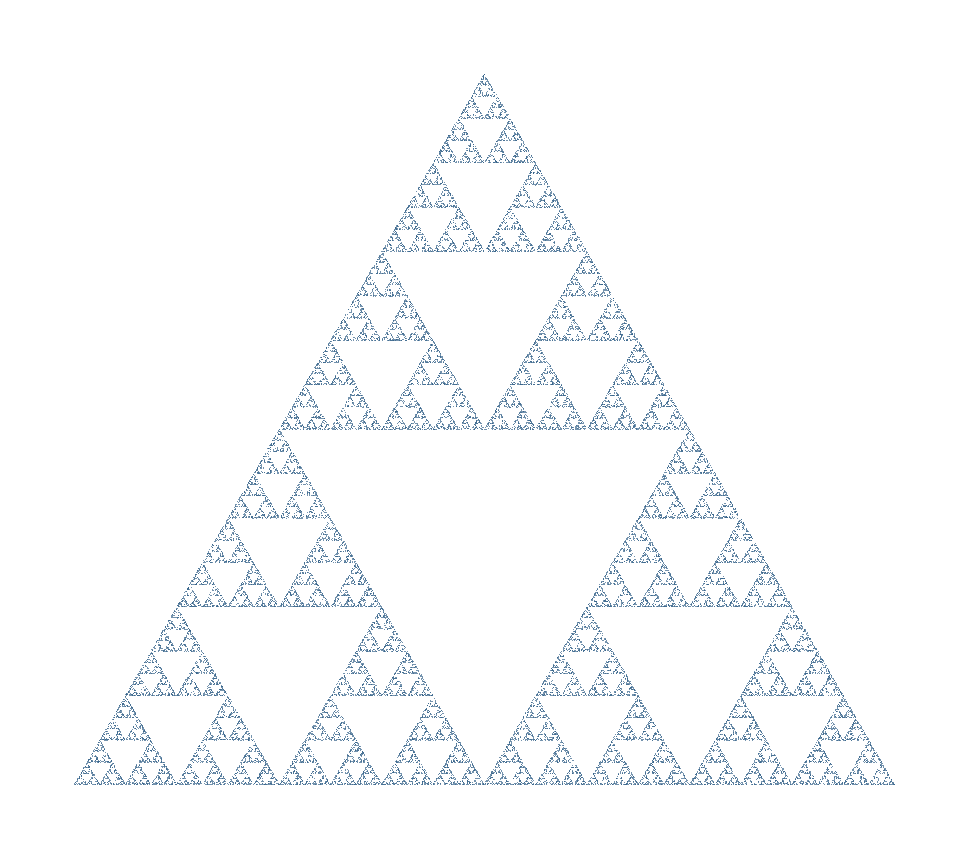
\includegraphics{py-sierpinski.png}}
    \end{column}
    \begin{column}{0.55\textwidth}
      \small
      Partant d'un point, on choisit au hasard, à répétition, l'un des
      trois sommets d'un triangle, et on avance à mi-chemin
      vers lui.
      \vspace{6pt}

      Pourquoi obtient-on toujours la même figure ?
      \begin{itemize}
        \item Réponse au chapitre 3, grâce au théorème du point
          fixe de Banach --- démontré aujourd'hui.
        \item La figure sera un point d'un espace dont les
          « points » sont des ensembles compacts du plan, muni de la
          distance de Hausdorff --- construite aujourd'hui.
      \end{itemize}
    \end{column}
  \end{columns}
\end{frame}

\begin{frame}{Le chemin de ce chapitre}
  \FigBox[0.42\textheight]{%
    \begin{tikzpicture}[
        etape/.style={draw=sectioncolor, fill=thmboxbg, rounded corners=2pt,
          thick, align=center, font=\scriptsize, minimum height=1.05cm,
          text width=2.05cm},
        but/.style={etape, draw=coveraccent!85!black, fill=secboxbg}]
      \node[etape] (m) at (0,0) {Métrique\\$(E,d)$};
      \node[etape] (o) at (2.6,0) {Ouverts, fermés,\\compacts};
      \node[etape] (h) at (5.2,0) {Distance de\\Hausdorff $\dH$};
      \node[etape] (c) at (2.6,-1.7) {Suites de Cauchy,\\complétude};
      \node[etape] (k) at (5.2,-1.7) {Points fixes,\\contractions};
      \node[but] (b) at (8.1,-0.85) {Théorème\\de Banach};
      \node[etape, text width=2.3cm] (n) at (11.0,0) {Méthode de\\Newton};
      \node[etape, text width=2.3cm] (f) at (11.0,-1.7) {Fractales\\(chapitre 3)};
      \draw[fleche] (m) -- (o);
      \draw[fleche] (o) -- (h);
      \draw[fleche] (m) |- (c);
      \draw[fleche] (c) -- (k);
      \draw[fleche] (k) -- (b);
      \draw[fleche] (h) -- (b);
      \draw[fleche] (b) -- (n);
      \draw[fleche] (b) -- (f);
    \end{tikzpicture}}
  \small Deux applications tout au long du chemin : la
  navigation sur une sphère et la détection d'erreurs
  dans une chaîne de bits.
\end{frame}
